\chapter{Conclusiones}

El \eyetracking web es un campo en sus primeros pasos de desarrollo pero que
suscita un creciente interés de distintos grupos.
Muchos de estos ya estaban explorando experimentos con \eyetracking web antes
del 2020 pero el aislamiento potenció y realzó su importancia.
En particular, el \eyetracking remoto gana mucho interés en el campo sustentado
en su amplia historia en el laboratorio, donde ha mostrado ser una ventana para
estudiar procesos cognitivos de forma no invasiva y con un contacto mínimo con
el sujeto experimental.
Nuestra pregunta original puede reformularse como hasta qué punto el
\eyetracking web puede reemplazar o extender a otros contextos el uso de
\eyetrackers tradicionales (en particular aquellos utilizados en laboratorio).
La implementación y experimentación realizadas sugieren un fuerte potencial
pero también muestran múltiples dificultades propias a este problema.

En el presente trabajo se replicaron los resultados generales esperados en la
tarea de antisacadas.
Las antisacadas incorrectas mostraron tiempos de respuesta menores que las
antisacadas correctas.
Esto es consistente con la noción de que realizar correctamente la tarea
implica un costo cognitivo adicional.
En la primera instancia de experimentación se obtuvo, para la tarea de
antisacadas, una tasa de correctitud dentro del rango esperable.
Mientras que en la segunda fue mayor, pero sí se comportó como era esperado ya
que fue mayor para el caso prosacada que para antisacada.

Como resultado de este trabajo se obtuvo un prototipo de \eyetracker web
utilizable en análisis clínicos remotos que permite obtener conclusiones de
alto nivel sobre el comportamiento del sujeto (e.g., a qué lado de la pantalla
mira el sujeto).
Este puede utilizarse en navegadores web a la par de \jspsych, provee
mecanismos de calibración y validación similares a aquellos de \eyetrackers
comerciales e incluye un mecanismo de detección de descalibraciones.
Se ofrece también la posibilidad de utilizar el prototipo a través de una
interfaz no dependiente de \jspsych.
En ambos casos se provee un \textit{playground} en los cuales se podrá
interactuar con las interfaces implementadas.
Además, se proveen criterios de exclusión y normalización para las estimaciones
obtenidas y mecanismos de detección de sacadas.

En el marco del trabajo, se realizó un análisis intuitivo sobre el rendimiento
de la implementación, el cual muestra frecuencias de muestreo menores a los 30
Hz y estimaciones con desviaciones respecto del punto real de la mirada, aunque
con correcto posicionamiento relativo (cf. sección
\ref{section:skewed-estimates}).
Además se adaptó a nuestras necesidades el modelo de estimación de la mirada de
\webgazer.
En líneas con los beneficios mencionados respecto de la existencia de
implementaciones abiertas, el código del prototipo y aquel de análisis de
estimaciones fue liberado en un repositorio público \footnote{repositorio
correspondiente a este trabajo:
\url{https://github.com/ffigari/rastreador-ocular}}, lo cual permitirá
realizar nuevas rondas de experimentación.
Las modificaciones sobre \webgazer se encuentran almacenadas en un
\textit{fork} propio \footnote{\textit{fork} propio de \webgazer:
\url{https://github.com/ffigari/WebGazer}}.
Este \textit{fork} se realizó desde el repositorio correspondiente al
\textit{fork} de \webgazer realizado por \jspsych \footnote{repositorio origen
del \textit{fork} propio de \webgazer:
\url{https://github.com/jspsych/WebGazer}}.
Al no estar estandarizado el reporte de errores en las herramientas de
\eyetracking \cite{zandi_2021_pupilext}, se dificulta comparar conclusiones de
distintos análisis clínicos.
Lo mismo ocurre cuando, en distintos trabajos se realizan implementaciones de
detección de sacadas propias \cite{salvucci_2000_identifying_fixations}.
En el campo de la oftalmología, para el caso de la perimetría automatizada
\cite{pubmed_1996_automated_perimetry}, aparece también esta dificultad para
comparar resultados obtenidos por distintas herramientas, aunque existen que
intentan compararlas \cite{landers_2007_automated_perimeters_comparison}.
Mientras que dentro de una misma herramienta se realizan incluso trabajos para
establecer valores normativos \cite{brenton_1986_humphrey_normal_visual_field}.
La existencia de una herramienta abierta para realizar estudios de movimientos
oculares online eliminaría a las diferencias implementativas como factor de
incompatibilidad.

\section{Limitaciones}

TODO: Chequear si las siguientes limitaciones están listadas en esta sección
- No está claro si el facemesh es ideal para localizar ojos, por ejemplo, se
está modelando toda la cara mientras que nos importa únicamente la posición de
un par de recuadros de los ojos.
No sólo parece excesivo en términos de costos computacionales, si no que al no
estar modelando específicamente los ojos sería esperable no obtener la mejor
precisión que podría obtenerse.
Existen en cambio mecanismos específicos para la localización de los ojos
\cite{hansen_2009_eye_of_the_beholder}.
- variabilidad e imprecisión en la duración de cada frame; molesto para cuando
se tien que mostrar un estímulo por poco tiempo (< 100 ms)



Se detectaron limitaciones tanto a nivel implementación como experimentación:
A nivel implementación: 

\begin{itemize}
  \item Las estimaciones tuvieron una frecuencia de muestreo promedio por
debajo de los 30 Hz para todos los sujetos, llegando incluso en algunos casos a
estar por debajo de los 5 Hz.
  En contraste, para \eyetrackers profesionales de laboratorio se reportan
frecuencias de muestreo de entre 100 Hz y 2000 Hz \cite{hosp_2020_remote_eye}.
  Para el \tobii se reporta una frecuencia de 133 Hz \footnote{especificaciones
de \tobii:
\url{https://help.tobii.com/hc/en-us/articles/360012483818-Specifications-for-Eye-Tracker-5}}
y para \eyelink una frecuencia máxima de 1000 Hz en el modo que permite mover
la cabeza \footnote{especificaciones de \eyelink:
\url{https://www.sr-research.com/wp-content/uploads/2017/11/eyelink-1000-plus-specifications.pdf}}.
\\
  La frecuencia máxima obtenible está limitada por la frecuencia del monitor
utilizado por el sujeto.
  Dado que los monitores modernos comerciales suelen tener al menos 60 Hz, esto
no explica por sí sólo la baja frecuencia obtenida. \\
  Al margen no haber terminado de dilucidar la razón de la baja frecuencia para
todas las variantes de hardware, ocurre que esta dificulta análisis posteriores
y, en particular, la implementación de una rutina de detección de sacadas.
  Lo cual implica un desafío en sí mismo.

  TODO: Reescribir el punto anterior

  \item En la implementación actual no se tuvieron en cuenta los pestañeos.
  Por un lado, esto posibilita la entrada de datos inválidos de calibración al
sistema.
  Podría ocurrir que el sujeto pestañee durante los instantes previos al
\textit{frame} que selecciona nuestra rutina de calibración.
  En caso de ocurrir esto, los datos de calibración estarían incluyendo
incorrectamente un \textit{frame} en el cual los ojos están cerrados, causando
ruido en el modelo interno de regresión.
  Por otro lado, experimentos informales \footnote{hilo de twitter:
\url{https://twitter.com/_HanZhang_/status/1527762369593606145}} muestran como
los pestañeos generan efectos negativos en las estimaciones.

  \item No se llegó a combinar el \eyetracking con una estimación de las
dimensiones del monitor.
  Por lo que las coordenadas de los estímulos presentados son indicadas en
píxeles.
  En la bibliografía es común, en cambio, reportar en grados de ángulo visual
tanto estos valores \cite{munoz_2004_look_away,
olincy_1997_age_diminishes_performance, smyrnis_2002_big_sample}, como errores
promedio \cite{huang_2016_pace, santini_2017_eyerectoo}.
  En consecuencia, sujetos que cuenten con pantallas de distintos tamaños y
resoluciones (cf. Figura \ref{fig:widths-distribution}) verán los
estímulos a distintos ángulos de visión.
  Esto podría ser un problema si un sujeto realiza el experimento en un monitor
con baja resolución o si está sentado considerablemente cerca de la pantalla.
  También podría aumentar la tendencia a mover la cabeza para observar los
estímulos laterales, facilitando así la descalibración del sistema.
\end{itemize}

A nivel experimentación: Al analizar los datos obtenidos, luego de aplicar las
rutinas de preprocesamiento se obtuvo una cantidad insuficiente de ensayos por
sujeto.
Esto puede deberse a 
\begin{itemize}
  \item Una rutina de preprocesamiento excesivamente exigentes.
  Mientras que en nuestro caso en ambas instancias se descartó aproximadamente
66\% de los ensayos, otros trabajos reportaron descartar menos del 2\%
\cite{unsworth_2011_distribution_analysis}. 

TODO: Revisitar el item siguiente cuando tenga mejor armada la explicación
      de detección de sacadas

  \item Tasas de correctitud muy elevadas.
  Por ejemplo, en la segunda instancia de experimentación se obtuvo una tasa de
correctitud de 95\% mientras que en la bibliografía se reportan valores
cercanos al rango [60\%, 70\%].
  Esto puede sugerir que ensayos incorrectos de la tarea son clasificados
incorrectamente como correctos.
  Y, a su vez, podría deberse a una incapacidad en detectar pequeñas sacadas
iniciales (cf. Figura \ref{fig:undetected-saccade-example}).
  Si bien se buscó implementar la rutina de detección de sacadas en base a
conceptos mencionados en la bibliografía (distancia recorrida, velocidad
promedio \cite{stuart_2019_saccade_detection_algorithms}) no se midió su
eficacia ni se comparó sus resultados contra otras implementaciones.
  En cualquier caso, la baja cantidad de ensayos incorrectos imposibilitó
realizar análisis por sujeto.
  Consecuentemente, no se pudo estudiar la capacidad de asistencia al
diagnóstico de la tarea de antisacadas en un contexto web remoto, lo cual era
uno de los objetivos iniciales del trabajo.

  \item Al momento de presentar la tesis no se logró la representatividad
esperada de distintos grupos etarios.
  Una hipótesis para esto es que la forma en la cual se distribuyó el
experimento no haya sido adecuada para alcanzar individuos de mayor edad (entre
50 y 80 años).
  En efecto, este tuvo que realizarse a través de un navegador web y fue
distribuido a través de redes sociales, lo cual parece más apropiado para
alcanzar poblaciones de menor edad (entre 20 y 35 años).
  Sumado a esto, ocurrió que todos los sujetos de entre 50 y 80 años (2 para la
primera instancia y 5 para la segunda instancia) fueron descartados durante el
preprocesamiento debido a bajas frecuencias de muestreo (cf. Figura
\ref{fig:sampling-frequencies-by-age}).
  Esto puede deberse a que las características del hardware utilizado también
se correlacionen con la edad.

  \begin{figure}
    \centering
    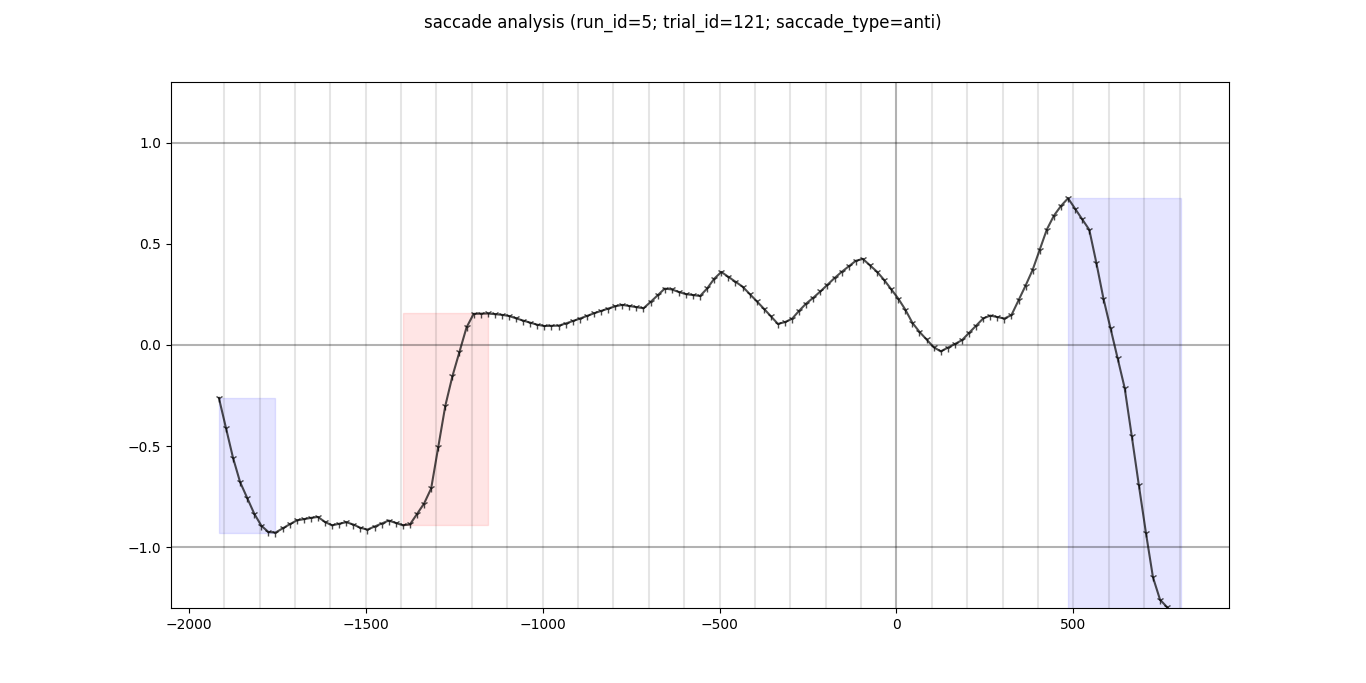
\includegraphics[width=\textwidth]{conclu/undetected-saccade-example.png}
    Se muestran arriba las estimaciones obtenidas (en negro) en cuatro ensayos.
    Los parches azules y rojos ilustran las sacadas detectas por nuestra
    rutina, azules siendo aquellas en dirección contraria al estímulo visual y
    rojas aquellas en misma dirección de este. \\
    TODO: Escribir esto dsp de decidir cómo explicar lo de los 0.6 minimo
    En los cuatro ejemplos presentados la rutina falló en detectar 


    se falla en reconocer la primer sacada
    en a y c esto resulta en dirección correcta pero con rt mayor al real
    en b y d 
    a y c ejemplifican dirección correcta detectada pero c

    [TODO: \\
    - Adjust style to be coherent with the informe \\
    - Comentar sobre las dos cosas distintas
      a) se falla en encontrar el lado correcto
      b) se reporta un tiempo de respuesta mayor del real]
    \caption{Sacadas no detectadas}
    \label{fig:undetected-saccade-example}
  \end{figure}

\end{itemize}

\section{Trabajo futuro}

El trabajo a futuro deberá avanzar sobre el desarrollo de la herramienta web y
sobre un esquema de análisis adaptado a ese tipo de datos. \\
Respecto del análisis de datos: 
\begin{itemize}
  \item Se deben buscar (o desarrollar) métodos de detección de sacadas capaces
de capturar pequeñas sacadas con las restricciones del \eyetracking web.
  Esto evitará, en el caso de la tarea de antisacadas, que se pasen por alto
pequeñas sacadas iniciales.
  Estas muchas veces iban en la dirección incorrecta y luego eran corregidas
con sacadas más grandes que si eran detectadas, aumentando la tasa de
correctitud.
  Para esto pueden, por ejemplo, buscarse los ensayos que se consideren
incorrectamente descartados. 

  \item En el mismo sentido se pueden revisar los criterios de exclusión.
  En la implementación actual, para conservar un ensayo es requisito que el
sujeto haya estado mirando al estímulo central de fijación durante los 500 ms
previos a la aparición del estímulo lateral.
  Sin embargo no se incluye un mecanismo de detección de fijaciones sino que se
verifica que durante ese período \begin{enumerate*}
    \item en promedio las estimaciones coincidan con el centro y
    \item no haya sacadas
\end{enumerate*}.
  Esto se puede mejorar implementando efectivamente mecanismos de detección de
fijaciones.
  También puede estudiarse si y cómo los criterios de filtrado modifican las
proporciones de cada población de sujetos, o si estos tienen por ejemplo mayor
tendencia a descartar ensayos que hubieran sido clasificados como incorrectos.
\end{itemize}

En base a estos puntos, también puede estimarse la tasa de ensayos que el
criterio descarta y elegirse adecuadamente la cantidad de ensayos que cada
sujeto debe realizar en futuros experimentos.

Además, se podría apuntar a conseguir mayor cantidad de sujetos, priorizando la
representatividad de distintos grupos etarios.
Con suficiente cantidad de datos se podrían estudiar las diferencias de edad
utilizando modelos Bayesianos multivariados
\cite{plomecka_2020_retest_reliability}, modelar los datos obtenidos con el
modelo SERIA (\textit{Stochastic Early Reaction, Inhibition, and late Action
model} \cite{aponte_2017_seria}) o realizar análisis de distribuciones sobre
los tiempos de respuesta \cite{unsworth_2011_distribution_analysis}.
Una dificultad no evidente de superar en este aspecto es la duración total del
experimento pues en simultáneo debe maximizarse la cantidad de ensayos por
experimento mientras también debe minimizarse su duración.
Cabe destacar cómo en la segunda instancia la mitad de los sujetos optó por
cortar tempranamente el experimento.

Respecto del desarrollo del \eyetracker: 
\begin{itemize}
  \item Se puede optimizar el prototipo tal que aumente la frecuencia de
muestreo.
  Para esto tienen que explorarse implementaciones alternativas de sus rutinas.
  Por ejemplo, 
  \begin{itemize}
    \item En el prototipo actual, la localización de los ojos depende de
generar un \textit{facemesh} por cada \textit{frame}, lo cual parece excesivo
pues luego se utiliza una fracción de tal información.
    Sin embargo, al existir métodos específicos a tal problema
\cite{hansen_2009_eye_of_the_beholder} sería esperable poder realizar
implementaciones más performantes. 

    \item Se podría realizar \textit{profiling} de la implementación presentada
para entender cuáles de sus elementos son los mayores causantes de la baja
frecuencia. 

    \item Se deberá estudiar en detalle cómo en un contexto de navegador pueden
capturarse los \textit{frames} de una webcam.
    La implementación actual se basa en el uso de \raf pero el
objetivo real de esta utilidad es sincronizarse con el refresco del monitor
para realizar animaciones, lo cual no es directamente relevante a nuestro
requisitos.
    De existir una forma alternativa de conectarse desde el navegador a la
webcam se podría desligar la implementación de tal utilidad.
    De esta manera el techo teórico de frecuencia de estimaciones estaría dado
por la frecuencia de muestreo de la webcam en lugar de por la tasa de refresco
del monitor.
  \end{itemize}

  \item Se deberá realizar experimentación donde se estudie la precisión
obtenible por el prototipo.
    Entre otros, puede estudiarse \begin{enumerate*}
      \item qué tan estáticas son las estimaciones mientras se sabe que el
        sujeto realiza una fijación,
      \item cuánto retraso existe entre que un sujeto reacciona y su registro
        en las estimaciones o
      \item de qué magnitud son y a qué se deben las desviaciones encontradas
        en la primera instancia de experimentación
    \end{enumerate*}.
  En el mismo sentido, durante una misma sesión de experimentación pueden
compararse las estimaciones del prototipo con estimaciones de \eyetrackers 
profesionales, como lo han hecho en otros trabajos de \eyetracking web
\cite{xu_2015_turker_gaze, huang_2016_pace}.
  Con una mayor comprensión de las precisiones alcanzables podrá luego
estudiarse qué información es extrapolable con las estimaciones.

  \item
    Otro aspecto del prototipo a explorar con mayor detalle es la
    detección de descalibraciones.
    Una primera opción es explorar modificaciones sobre la detección de
    movimiento en la cual esta esta basada.
    Por ejemplo, puede modificarse el factor de cambio de tamaño de los
    recuadros del ojo (figura \ref{fig:features-to-stillness-region}) y
    estudiar el impacto en la notificación de descalibraciones.
    Es esperable también poder detectar descalibraciones sin recurrir a
    detección de movimiento.
    Por ejemplo, \eyetrackers comerciales muestran regularmente un punto para
    detectar si la estimación en ese momento coincide con las coordenadas del
    punto (e.g., \textit{drift correction} en el \eyetracker \eyelink).
    Al momento de implementar alguno de estos mecanismos debe tenerse en cuenta
    su rendimiento y cómo se vea afectada la duración total del experimento. \\
    Al margen de cómo se implemente la detección de descalibración, debe
    definirse con mayor claridad qué significa que la herramienta esté
    correctamente calibrada.
    Como ha mostrado nuestra experimentación, es posible que las estimaciones
    arrojadas por la herramienta no coincidan con la mirada real pero que aun
    así pueda extrapolarse información.
    La definición de calibración está entonces ligada a la pregunta que se
    busca responder.
    Si como en nuestro caso alcanza con poder discernir la posición relativa de
    las estimaciones a lo largo del tiempo, entonces sería esperable poder
    relajar el criterio de descalibración actual.
    Similarmente, en el concepto de calibración debería considerarse la
    granularidad espacial deseada para las estimaciones.
    En nuestro caso alcanzó con distinguir tres regiones de interés (centro,
    izquierda y derecha) pero en otros problemas (e.g., rastreo de la atención
    durante una tarea de lectura) serán deseables mayores niveles de precisión.

  \item Es esperable poder encontrar rutinas más sofisticadas para la
calibración que la rutina actual.
  Como se ha detallado en la introducción de este informe, la implementación de
esta implica múltiples pequeñas decisiones de diseño.
  Para cada una de ellas aplica probar alternativas y estudiar cómo esto afecta
el rendimiento.
  Siguiendo las líneas de otros trabajos de \eyetracking web, puede buscar
capturarse el \textit{frame} de mayor coincidencia entre mirada y posición del
estímulo presentado \cite{huang_2016_pace} o bien probar utilizar varios
\textit{frames} por estímulo y descartar aquellos en los cuales ocurra un
pestañeo \cite{xu_2015_turker_gaze}. 

  \item Un último punto relacionado a la calibración es permitir generar
correctas estimaciones en regiones de interés más allá de aquellas tres
relevantes a la tarea de antisacadas.
  En efecto, la implementación presentada está limitada en no poder ser
utilizada para estudiar comportamiento sobre el eje vertical.
  Aplica entonces ser capaz de elegir las regiones de interés en función del
experimento que se desea realizar.

  \item En futuras implementaciones los pestañeos deben ser continuamente
detectados.
  Si bien no se ha hecho un análisis detallado al respecto, es esperable que
estos generen ruido significativo sobre las estimaciones.
  Es necesario entonces reportar los períodos de pestañeos para que estos
puedan ser considerados en subsecuentes análisis de las estimaciones.

  \item Respecto de la precisión espacial, en el laboratorio se ha desarrollado
un \textit{plugin} para \jspsych que permite conocer en cada sesión la relación
entre cantidad de píxeles y cantidad de grados de visión (\textit{virtual
chinrest} \cite{li_2020_virtual_chinrest}).
  Esto posibilita presentar los estímulos de calibración y aquellos de la tarea
de antisacadas en función del ángulo de la mirada, que tal como se mencionó
suele ser la forma habitual de reportar estas distancias en la bibliografía.
  La implementación puede extenderse tal que estén codificados tanto en grados
como en píxeles, utilizando el valor en grados cuando el \textit{plugin} esté
presente.

  \item También sería importante implementar verificaciones sobre las
condiciones iniciales del entorno, así como también pedidos de ajustes sobre
ella e incluso barreras de requerimientos tal que de no ser cumplidas no se
permita proseguir con el experimento.
  Por ejemplo, en \turkergaze se solicita al sujeto ajustar la iluminación del
ambiente de ser esta inadecuada.
  Otros posibles objetos de verificación incluyen la resolución de la cámara
web, la resolución del monitor o el posicionamiento del sujeto en relación a la
cámara.
\end{itemize}


Al margen de las implementaciones existentes, debe tenerse en cuenta como la
bibliografía existente no suele aplicar al contexto web.
Por ejemplo, gran parte de los métodos de modelado de la mirada asumen
capacidades de hardware y de modificación sobre el entorno que no son posibles
en este contexto \cite{hansen_2009_eye_of_the_beholder}.
Antoniades et al \cite{antoniades_2013_standarized_protocol} han presentado un
estándar de protocolo para la tarea de antisacadas, pero este sugiere
frecuencias de muestreo no alcanzables en contextos web.
Tampoco tienen en consideración la necesidad de mostrar las instrucciones del
experimento a su inicio en lugar de que estas sean indicadas por un
experimentador, lo cual es esperable que alargue la duración final del
experimento. 

En resumen, es necesario revisar el problema de estimación de la mirada de
principio a fin para entender en qué lugares debe profundizarse la
bibliografía.
Esto incluye a los modelos principales de localización de los ojos y de
modelado de la mirada, pero también a todo mecanismo circundante como son la
detección de sacadas o las rutinas de calibración.
En tal búsqueda debe tenerse en cuenta que tales métodos serán implementados en
\js de navegador, lo cual puede presentar dificultades propias.

Las limitaciones del contexto web encontradas hasta el momento indicarían que
el \eyetracking web puede ser utilizado en un subconjunto de los problemas
atacables por el \eyetracking tradicional de laboratorio.
Sin embargo, su fácil distribución así como la ausencia de costos de hardware y
potencialmente de software podrían presentar nuevas oportunidades.
Sumado a un estudio de la precisión y del rendimiento alcanzables, es preciso
entender en qué categorías de problemas puede utilizarse \eyetracking web.
Por lo pronto, problemas conocidos que requieren \eyetracking como la
generación de mapas de saliencia \cite{xu_2015_turker_gaze}, el modelado de la
búsqueda visual \cite{clifton_2016_eye_movements_in_reading} o el estudio de la
atención durante la lectura [50.3] podrían combinarse con
\textit{crowdsourcing} para alcanzar mayor cantidad y variabilidad de
poblaciones.
